\documentclass[10pt,journal]{IEEEtran}
\usepackage{amsmath,amssymb,booktabs,graphicx,array}
\usepackage[T1]{fontenc}
\usepackage{xcolor}
\usepackage[hidelinks]{hyperref}
\usepackage{fancyhdr}
\usepackage{lmodern}
\hyphenpenalty=10000
\exhyphenpenalty=10000
\tolerance=3000
\emergencystretch=3em
\renewcommand{\IEEEiedlistdecl}{\IEEEsetlabelwidth{SS}}

\fancypagestyle{plain}{\fancyhf{}\renewcommand{\headrulewidth}{0pt}\fancyhead[C]{\footnotesize\thepage}\fancyfoot[C]{\footnotesize\textbf{\textcopyright\ Nov 2026 Ahnaf A.G. $\mid$ Institut Teknologi Sepuluh Nopember}\\ \href{https://github.com/ahnafyura/webots-obstacle-avoidance-b401}{\textcolor{blue}{\underline{https://github.com/ahnafyura/webots-obstacle-avoidance-b401}}}}}
\pagestyle{plain}
\begin{document}

\title{Joint Space Trajectory Generation and Servo Tracking for Humanoid NAO Locomotion in Webots}

\author{Ahnaf Al Ghiffarri Ahtasyafi\\
\textit{Department of Computer Engineering, Institut Teknologi Sepuluh Nopember (ITS), Surabaya, Indonesia}}

\maketitle
\thispagestyle{plain}

\noindent\textbf{\textit{Abstract.}} Humanoid locomotion in simulation is often reduced to a sequence of keyframes sent to joint motors, and the budgets that make such a sequence feasible for the servos are rarely written down. This paper treats the joint level motion generator of a NAO humanoid in Webots as a composition of four operators on a joint state trajectory and derives three design tools for it. The first is a velocity utilization index with a time scaling bound and a closed form minimum blend duration. The second is a spectral bandwidth budget, which shows that the servo bandwidth needed for an RMS tracking error $\varepsilon$ is approximately $2\dot q_{\mathrm{rms}}/\varepsilon$. The third is a turning law for a hip yaw pulse. Applied to the walking clip shipped with Webots, the analysis shows that the right knee uses 102 percent of its velocity limit, so the clip cannot be sped up, that the clip energy concentrates at the stride frequency of 0.98 Hz, that only 10 of the 22 joints move, and that about 70 to 110 rad/s of servo bandwidth keeps the knee within 2 to 3 degrees RMS. Kinematic chain, joint state tensor, and phase portrait views make the joint indices, axes, and states explicit. A planar forward kinematics model predicts the stride length within 11 percent. In an automated test of 32 runs and 5.3 hours of simulated time the resulting controller had no collisions and no falls.

\vspace{2pt}
\noindent\textbf{\textit{Index Terms.}} Humanoid robot, NAO, Webots, joint space trajectory, servo control, gait generation.

\section{Introduction}
Position controlled humanoids such as NAO receive a vector of joint angle targets at every control step and rely on the joint servos to reach them \cite{gouaillier2009}. A walking controller therefore reduces to a function that maps time to a joint angle vector. Two failure modes are common. The first is a discontinuity, for example when a recorded motion starts from a pose that differs from the current posture, which asks the servo for an unbounded velocity. The second is a mismatch between the frequency content of the command and the bandwidth of the servo, which produces tracking lag that shifts the center of mass.

Much of the humanoid literature addresses the layer above this one, namely footstep planning, the Zero Moment Point criterion and its reference generation \cite{vukobratovic2004,erbatur2009}, preview control of a linear inverted pendulum \cite{kajita2003,kajita2010}, hybrid zero dynamics \cite{westervelt2003}, and divergent component of motion \cite{englsberger2015}. Those methods output a center of mass or foot reference that must still be converted into joint angles, typically with the analytical inverse kinematics of NAO \cite{kofinas2015}. The conversion and the servo that follows it are treated here.

Other work optimizes the timing of a given path under velocity and torque limits \cite{bobrow1985,pham2018}. Within the sources cited here we did not find an analysis that takes an already recorded motion clip and returns, in closed form, its velocity margin, the shortest feasible transition between poses, and the servo bandwidth it requires. That replay layer is the subject of this paper. The scope is deliberate. The results are analytical tools together with a case study, not a new walking controller.

The study is based on a working Webots controller in which a NAO walks in a five by five meter arena with twelve obstacles. Its gait engine does not use inverse kinematics. It replays and modifies the walking clip distributed with Webots and commands every joint through the position interface of the simulator \cite{michel2004}. The contributions are as follows.
\begin{enumerate}
\item A compact operator formulation of the gait engine on a joint state trajectory, with the properties of each operator derived in closed form, including a proof that smoothstep blending minimizes acceleration energy \cite{flash1985}.
\item A velocity utilization index with a uniform time scaling bound and a closed form minimum synchronized blend duration, which is a special case of time optimal path parameterization \cite{bobrow1985,pham2018}.
\item A spectral bandwidth budget $\omega_n^{*}\approx2\dot q_{\mathrm{rms}}/\varepsilon$ that links the RMS joint velocity of a clip to the servo bandwidth it requires, checked against the exact value to within 10 percent.
\item An empirical turning law for the hip yaw pulse and for yaw scaling, including a measured left right asymmetry.
\item Joint state views, namely a kinematic chain with indices, roles, axes, and states, a joint state tensor, and phase portraits, applied to the Webots walking clip.
\item A reconciliation of the analysis with simulation measurements from the same controller.
\end{enumerate}
All numbers computed from the motion files can be reproduced with the analysis scripts that accompany this paper. Quantities that depend on the servo gains of the simulated robot are treated as parameters, because those gains were not inspected in this study.

\section{Robot and Joint Model}
The controller commands $n=22$ joints, namely two head joints, eight arm joints, and six joints in each leg. The leg chain is Hip Yaw Pitch, Hip Roll, Hip Pitch, Knee Pitch, Ankle Pitch, and Ankle Roll, following the Denavit and Hartenberg convention \cite{denavit1955}. From the Webots URDF export the thigh length is $L_1=0.100$ m, the shank length is $L_2=0.1029$ m, and the hip is offset by $(0,\,0.05,\,-0.085)$ m from the torso frame. The velocity limits are 6.40 rad/s for the pitch joints and 4.16 rad/s for the roll and yaw joints, and the effort limits are 9.8 N m and 14.8 N m respectively. The two hip yaw pitch joints use an inclined axis $(0,\,1/\sqrt{2},\,-1/\sqrt{2})$, which is the mechanical coupling described in \cite{kofinas2015}.

\subsection{Joint indices and state}
The joints are indexed $n=1,\dots,22$ in the order left leg ($n=1$ to $6$), right leg (7 to 12), left arm (13 to 16), right arm (17 to 20), and head (21 and 22). The state of joint $n$ is $\mathbf{x}_n=[q_n,\dot q_n]^{\top}$, the full state is $\mathbf{x}\in\mathbb{R}^{44}$, and a clip of $N$ frames is stored as the joint state tensor $\mathbf{Q}\in\mathbb{R}^{22\times N}$ with entries $Q_{nk}=q_n(t_k)$. Each joint has a role, Roll, Pitch, or Yaw, given by its name, and a local rotation axis $\mathbf{a}_n$ in the URDF frame, with $x$ forward, $y$ left, and $z$ up in the base frame. Figure~\ref{fig:kin} lists the indices, roles, axes, and states of the left leg, left arm, and head, and shows the left leg in the base frame.

\begin{figure*}[t]
\centering
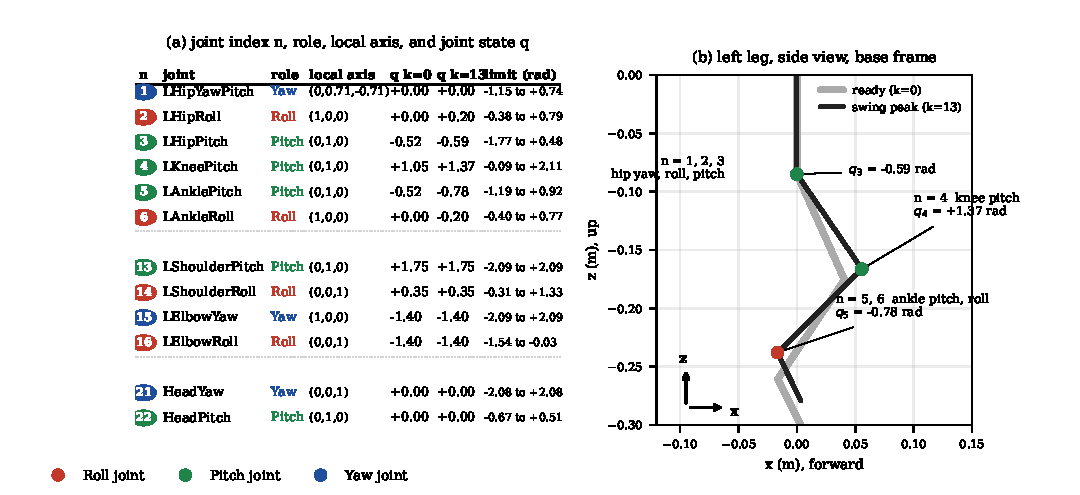
\includegraphics[width=\textwidth]{fig/f_kin3d.pdf}
\caption{Kinematic chain of NAO as controlled in Webots. Panel (a) gives the index $n$, role, local axis, state at frames 0 and 13 of the loop, and limits of the left leg, left arm, and head. The right side is the mirror image. Panel (b) shows the left leg in the sagittal plane of the base frame at the ready posture and at the swing peak.}
\label{fig:kin}
\end{figure*}

\subsection{Sagittal forward kinematics}
Let $\theta_h$, $\theta_k$, and $\theta_a$ be the hip, knee, and ankle pitch angles. With the sign convention of the model, the thigh angle from the vertical is $\phi_1=-\theta_h$, the shank angle is $\phi_2=\phi_1-\theta_k$, and the foot angle is $\phi_3=\phi_2-\theta_a$. The ankle position relative to the hip in the sagittal plane is
\begin{equation}
\begin{aligned}
x &= L_1\sin\phi_1 + L_2\sin\phi_2,\\
z &= -\left(L_1\cos\phi_1 + L_2\cos\phi_2\right).
\end{aligned}
\label{eq:fk}
\end{equation}
The sole stays parallel to the ground when
\begin{equation}
\theta_h+\theta_k+\theta_a = 0 .
\label{eq:flat}
\end{equation}
The ready posture used by the controller has $\theta_h=-0.524$, $\theta_k=1.047$, and $\theta_a=-0.524$ rad, so the left side of \eqref{eq:flat} equals $-0.001$ rad and the ankle sits $0.176$ m below the hip, which is 87 percent of the straight leg length of $0.2029$ m. This bent knee posture lowers the center of mass and is the starting point of every motion.

\section{Joint Trajectory Generation}
Let $\mathbf{q}(t)\in\mathbb{R}^{n}$ be the commanded joint vector and $h$ the control step. The gait engine builds $\mathbf{q}(t)$ from four operators.

\subsection{Keyframe interpolation}
The Webots motion format stores poses $\mathbf{q}_k$ at the times $t_k=kh_m$ with $h_m=0.04$ s. The engine interpolates linearly,
\begin{equation}
\mathbf{q}(t)=\mathbf{q}_k+\frac{t-t_k}{h_m}\left(\mathbf{q}_{k+1}-\mathbf{q}_k\right),\quad t_k\le t<t_{k+1}.
\label{eq:lin}
\end{equation}
If the underlying motion is twice differentiable, the interpolation error obeys $\lVert\mathbf{q}(t)-\mathbf{q}_{true}(t)\rVert_\infty\le \tfrac{h_m^2}{8}\max\lvert\ddot{\mathbf{q}}\rvert$. Applied to the finite difference acceleration of the walking clip this gives at most $1.07^\circ$, $1.15^\circ$, and $0.97^\circ$ for the hip, knee, and ankle pitch joints, which is small against the motion range of about $29^\circ$ to $38^\circ$.

\subsection{Smoothstep blending}
Playing a stored clip from the current posture requires a bridge from the last target $\mathbf{q}_a$ to the first pose $\mathbf{q}_b$ of the clip. The engine uses
\begin{equation}
\mathbf{q}(t)=\mathbf{q}_a+\left(\mathbf{q}_b-\mathbf{q}_a\right)\sigma\!\left(\frac{t}{T_b}\right),\quad \sigma(u)=3u^2-2u^3,
\label{eq:smooth}
\end{equation}
with $T_b=0.4$ s by default and $1.2$ s for the initial transition to the ready posture.

\medskip
\noindent\textbf{Proposition 1.} Among all twice differentiable paths $q(t)$ on $[0,T]$ with $q(0)=a$, $q(T)=b$, and $\dot q(0)=\dot q(T)=0$, the smoothstep path \eqref{eq:smooth} minimizes $\int_0^T\ddot q^{\,2}\,dt$.

\medskip
\noindent\textit{Proof.} The Euler Lagrange equation of the functional is $q^{(4)}(t)=0$, so the minimizer is a cubic polynomial. The four boundary conditions determine its four coefficients, and $a+(b-a)\sigma(t/T)$ satisfies all of them. The functional is convex, so the stationary point is the global minimum. $\square$

The derivatives of $\sigma$ are $\sigma'(u)=6u(1-u)$, $\sigma''(u)=6-12u$, and $\sigma'''(u)=-12$. For a displacement $\Delta=\lvert b-a\rvert$ over a duration $T$, the peak velocity is therefore $\tfrac{3\Delta}{2T}$ at the midpoint, the peak acceleration is $\tfrac{6\Delta}{T^2}$ at the two ends, and the jerk is constant at $\tfrac{12\Delta}{T^3}$ in magnitude with a jump at the ends. The path is $C^1$ but not $C^2$.

The quintic profile $\sigma_5(u)=10u^3-15u^4+6u^5$ minimizes the squared jerk integral for the same position and velocity conditions plus zero end acceleration \cite{flash1985}. Table~\ref{tab:profiles} compares the profiles, and Fig.~\ref{fig:blend} shows them. The quintic is smoother in acceleration, but it demands a 25 percent higher peak velocity than smoothstep, and for servos that are velocity limited the cubic is the more conservative choice.

\begin{table}[t]
\centering
\caption{Normalized peaks for a unit displacement over a unit time}
\label{tab:profiles}
\small
\begin{tabular}{lccc}
\toprule
Profile & Peak vel. & Peak acc. & End acc.\\
\midrule
Linear & 1.000 & unbounded & undefined\\
Smoothstep & 1.500 & 6.000 & nonzero\\
Quintic & 1.875 & 5.773 & zero\\
\bottomrule
\end{tabular}
\end{table}

\begin{figure}[t]
\centering
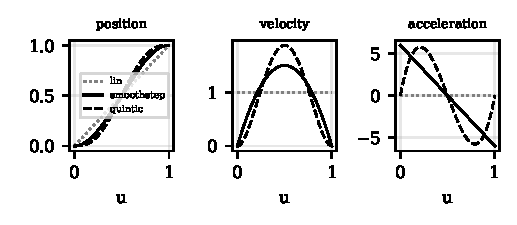
\includegraphics[width=\columnwidth]{fig/f_blend.pdf}
\caption{Position, velocity, and acceleration of the linear, smoothstep, and quintic profiles on the unit interval.}
\label{fig:blend}
\end{figure}

\subsection{Cyclic closure}
A walking cycle can be repeated without a seam only if the clip is closed. The controller cuts frames 51 to 102 of the Webots clip \texttt{Forwards50}, a loop of $N=51$ intervals and $T_c=2.04$ s. Closure requires $\mathbf{q}(T_c)=\mathbf{q}(0)$, and the measured defect is $\max_j\lvert q_j(T_c)-q_j(0)\rvert=0$ rad for all joints. Velocity closure is weaker. Because \eqref{eq:lin} is piecewise linear, the velocity at the seam jumps by 0.23, 0.33, and 0.10 rad/s for the hip, knee, and ankle pitch joints, which is less than 6 percent of the velocity limit in every case.

\subsection{Hip yaw pulse for turning while walking}
Turning is obtained by adding a pulse to both Hip Yaw Pitch joints over one cycle. With the frame boundaries $(a,b,c)=(7,20,33)$ for a left turn and $(20,33,46)$ for a right turn, and $s_k$ defined piecewise,
\begin{equation}
s_k=\begin{cases}
(k-a)/(b-a), & a\le k<b,\\
1-(k-b)/(c-b), & b\le k<c,\\
0, & \text{otherwise,}
\end{cases}
\label{eq:pulse}
\end{equation}
and the update $q_{\mathrm{yaw},k}\leftarrow q_{\mathrm{yaw},k}-A\,\sigma(s_k)$ with $A=0.25$ rad. The pulse is zero at the cycle boundary, so the closure of the clip is preserved. Its rise time is $13h_m=0.52$ s, hence the peak velocity is $\tfrac{3A}{2\cdot0.52}=0.72$ rad/s, which uses 17 percent of the yaw velocity limit.

For turning in place, the clip yaw joints are scaled by a factor $\kappa$, $q_{\mathrm{yaw}}\leftarrow\kappa\,q_{\mathrm{yaw}}$. Section~\ref{sec:valid} shows that the resulting heading change is nearly linear in $\kappa$.

\subsection{Composition}
Let $\mathcal{B}$, $\mathcal{C}$, $\mathcal{P}$, and $\mathcal{S}_\kappa$ denote blending, cyclic extension, the yaw pulse, and yaw scaling. The command for a walking left turn is $\mathbf{q}=\mathcal{B}\bigl(\mathcal{C}(\mathcal{P}(\text{loop}))\bigr)$ at the start and $\mathcal{C}(\mathcal{P}(\text{loop}))$ afterwards. Blending is skipped between clips that belong to the same cycle family, because their poses coincide at the seam.

\section{Velocity Feasibility and Minimum Blend Time}
Let $\bar v_n$ be the velocity limit of joint $n$ and define the velocity utilization index
\begin{equation}
\mathrm{VUI}_n=\frac{\max_t\lvert\dot q_n(t)\rvert}{\bar v_n},\qquad \mathrm{VUI}=\max_n\mathrm{VUI}_n .
\label{eq:vui}
\end{equation}

\medskip
\noindent\textbf{Proposition 2.} Playing a clip at the speed factor $\lambda$, that is $q_\lambda(t)=q(\lambda t)$, is velocity feasible if and only if $\lambda\le\lambda_{\max}=1/\mathrm{VUI}$.

\medskip
\noindent\textit{Proof.} The velocity scales as $\dot q_\lambda(t)=\lambda\dot q(\lambda t)$, so $\max_t\lvert\dot q_{\lambda,n}\rvert=\lambda\,\mathrm{VUI}_n\bar v_n$ and the constraint holds for all joints exactly when $\lambda\,\mathrm{VUI}\le1$. $\square$

\medskip
\noindent\textbf{Proposition 3.} A smoothstep blend \eqref{eq:smooth} with one shared duration $T_b$ for all joints and displacements $\Delta_n=\lvert q_{b,n}-q_{a,n}\rvert$ satisfies the velocity limits if and only if
\begin{equation}
T_b\ge T_b^{*}=\max_n\frac{3\Delta_n}{2\bar v_n}.
\label{eq:tstar}
\end{equation}

\medskip
\noindent\textit{Proof.} The peak velocity of joint $n$ is $3\Delta_n/(2T_b)$ from Section III, and requiring it to be at most $\bar v_n$ for every $n$ gives \eqref{eq:tstar}. A shared duration keeps all joints arriving together, so the blend is a straight line in joint space. $\square$

Both propositions are special cases of time optimal path parameterization \cite{bobrow1985,pham2018} with velocity constraints only and a constant or cubic speed profile. Their value here is that they need no optimization and can be evaluated from a clip in one pass.

The walking loop has $\mathrm{VUI}=1.023$ at the right knee, so $\lambda_{\max}=0.977$. The clip is already at the edge of what the joints can do, and the mean walking speed of 0.088 m/s cannot be raised by playing it faster. A faster walk needs a clip with a different stride, not a time scaling. Table~\ref{tab:tstar} gives $T_b^{*}$ for the transitions used by the controller. The initial move to the ready posture is limited by the left shoulder pitch, which has a displacement of 1.745 rad and a velocity limit of 8 rad/s, giving $T_b^{*}=0.327$ s against the 1.2 s used. The blend from the ready posture to the first pose of the walking clip is limited by the left knee at 0.041 s against 0.4 s used. The other transitions need less than 0.010 s. These values are lower bounds from velocity alone, since torque and balance demand more, so the ratio in Table~\ref{tab:tstar} is a margin and not a recommendation to shorten the blends.

\begin{table}[t]
\centering
\caption{Minimum blend duration from \eqref{eq:tstar} against the duration used}
\label{tab:tstar}
\footnotesize
\setlength{\tabcolsep}{3pt}
\begin{tabular}{lcccc}
\toprule
Transition & Limiting joint & $T_b^{*}$ (s) & Used (s) & Ratio\\
\midrule
Stand to ready & L shoulder & 0.327 & 1.2 & 3.7\\
Ready to walk start & L knee & 0.041 & 0.4 & 9.8\\
Ready to other clips & L hip roll & under 0.01 & 0.4 & over 40\\
\bottomrule
\end{tabular}
\end{table}

\section{Servo Tracking Model}
In Webots the target $q_c$ is passed to the motor with the position interface, and the simulator closes a PID loop around the joint, limited by the maximum velocity and available torque of the motor \cite{webotsmanual}. For a joint with inertia $J$ and damping $b$ the PD part of the loop gives, neglecting load and the integral term,
\begin{equation}
H(s)=\frac{K_d s+K_p}{Js^2+(b+K_d)s+K_p}.
\label{eq:H}
\end{equation}
A PID of this kind remains the dominant industrial structure \cite{astrom2001}. The gains of the NAO model were not read in this study, so $H(s)$ is approximated by a critically damped second order system with natural frequency $\omega_n$, $H(s)=\omega_n^2/(s+\omega_n)^2$. For a periodic command with harmonics $a_k\cos(k\omega_0 t+\varphi_k)$ and $\omega_0=2\pi/T_c$, the steady state tracking error has the amplitude $\lvert 1-H(jk\omega_0)\rvert\,a_k$ in each harmonic, and the RMS error is
\begin{equation}
e_{\mathrm{rms}}=\sqrt{\tfrac12\sum_{k\ge1}\lvert 1-H(jk\omega_0)\rvert^2a_k^2}.
\label{eq:erms}
\end{equation}
At low frequency $1-H(j\omega)\approx 2j\omega/\omega_n$, which gives the lag bound $e\le \tfrac{2}{\omega_n}\max\lvert\dot q\rvert$.

The velocity limit $\bar v$ adds a saturation. For a command with $\lvert\dot q_c\rvert>\bar v$ over an interval, the ideal slew limited servo $\dot q=\mathrm{sat}_{\bar v}\bigl(\dot q_c\bigr)$ accumulates a deviation of at most $\int(\lvert\dot q_c\rvert-\bar v)^+dt$.

\subsection{Spectral bandwidth budget}
For the critically damped model the error factor has the closed form $\lvert1-H(j\omega)\rvert=\omega\sqrt{\omega^2+4\omega_n^2}\,/\,(\omega_n^2+\omega^2)$, which tends to $2\omega/\omega_n$ when $\omega\ll\omega_n$. Substituting into \eqref{eq:erms} and using Parseval's identity for the periodic clip, $\dot q_{\mathrm{rms}}^{2}=\tfrac12\sum_{k\ge1}(k\omega_0a_k)^2$, gives
\begin{equation}
e_{\mathrm{rms}}\approx\frac{2\,\dot q_{\mathrm{rms}}}{\omega_n}
\quad\Longrightarrow\quad
\omega_n^{*}(\varepsilon)\approx\frac{2\,\dot q_{\mathrm{rms}}}{\varepsilon}.
\label{eq:budget}
\end{equation}
The servo bandwidth needed for a tolerance $\varepsilon$ is therefore set by the RMS velocity of the clip alone, and no spectrum is needed. Section~\ref{sec:analysis} compares \eqref{eq:budget} with the exact root of \eqref{eq:erms}.

\section{Analysis of the Walking Clip}
\label{sec:analysis}
\subsection{Velocity utilization}
Table~\ref{tab:util} lists the range of motion and the peak velocity of the left leg joints of the loop, with the peaks computed from finite differences at $h_m$. The knee reaches 6.42 rad/s on the left and 6.55 rad/s on the right, which is 100 and 102 percent of the limit of 6.40 rad/s, and the hip pitch reaches 93 percent. The overshoot above 100 percent is a property of the piecewise linear command and is not physically realizable by the servo. Simulating an ideal slew limited servo at the 20 ms control step gives a maximum deviation of $0.05^\circ$ for the left knee and $0.34^\circ$ for the right knee, so the saturation is harmless in practice. The consequence is that the knee has no velocity margin, and any modification that scales this clip in time must slow it down, not speed it up. The blend of the controller never contributes to the demand, since the worst case blend from the ready posture to the first pose of the clip has a peak velocity of only 0.66 rad/s and a peak acceleration of 6.6 rad/s$^2$, compared with in cycle accelerations of about 100 rad/s$^2$.

\begin{table}[t]
\centering
\caption{Left leg joint statistics of the walking loop. Range in rad, velocity in rad/s, acceleration in rad/s$^2$}
\label{tab:util}
\small
\begin{tabular}{lcccc}
\toprule
Joint & Range & Peak vel. & Util. & Peak acc.\\
\midrule
Hip Roll & 0.33 & 1.72 & 0.41 & 36\\
Hip Pitch & 0.66 & 5.98 & 0.93 & 94\\
Knee Pitch & 0.56 & 6.42 & 1.00 & 101\\
Ankle Pitch & 0.50 & 3.50 & 0.55 & 84\\
Ankle Roll & 0.38 & 1.72 & 0.41 & 21\\
\bottomrule
\end{tabular}
\end{table}

\begin{figure}[t]
\centering
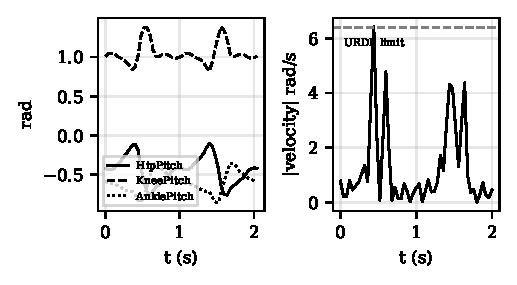
\includegraphics[width=\columnwidth]{fig/f_siklus.pdf}
\caption{Left leg pitch joint angles over the 2.04 s loop (left) and the knee velocity against the velocity limit of the model (right).}
\label{fig:cycle}
\end{figure}

\subsection{Spectral content}
Because the loop is periodic, its Fourier series is exact. Figure~\ref{fig:fourier} shows the first six harmonics. The first and third harmonics are below 0.01 rad in every pitch and roll joint, and the energy sits at the even harmonics. This follows from the structure of the clip, which holds two nearly identical gait periods of 1.02 s, so the dominant frequency is the stride frequency $f_s=2/T_c=0.98$ Hz. At $k=2$ the amplitudes are 0.199 rad for the hip pitch, 0.092 rad for the knee, and 0.150 rad for the ankle pitch. The knee is the least compact joint, since its fourth harmonic of 0.119 rad exceeds its second. The first five harmonics hold 92.5 percent of the alternating energy of the hip, 66.0 percent for the knee, and 88.9 percent for the ankle. The two roll joints are almost pure tones, with 97.6 percent and 99.8 percent of their energy in the first three harmonics. A servo that follows the stride frequency and its first two multiples (up to about 3 Hz) therefore captures most of the command.

\begin{figure}[t]
\centering
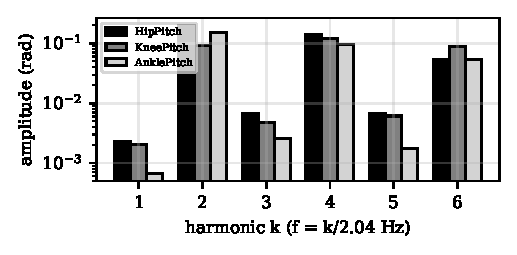
\includegraphics[width=\columnwidth]{fig/f_fourier.pdf}
\caption{Fourier amplitudes of the left leg pitch joints, harmonic $k$ corresponds to the frequency $k/2.04$ Hz.}
\label{fig:fourier}
\end{figure}

\subsection{Servo bandwidth requirement}
Evaluating \eqref{eq:erms} with the measured harmonics gives Table~\ref{tab:servo} and Fig.~\ref{fig:servo}. The RMS error is dominated by the phase lag at the stride frequency. A bandwidth of 20 rad/s leaves 5.8 to 7.8 degrees of RMS error, 40 rad/s leaves 3.6 to 4.8 degrees, and 80 rad/s leaves 2.0 to 2.7 degrees. Since the limiting behavior is $e_{\mathrm{rms}}\propto 1/\omega_n$, halving the error costs a doubling of the servo bandwidth. These values are the sensitivity of the clip to the servo, and they are model results, not Webots measurements.

\begin{table}[t]
\centering
\caption{RMS tracking error (degrees) of the clip for a critically damped servo model}
\label{tab:servo}
\small
\begin{tabular}{lccc}
\toprule
$\omega_n$ (rad/s) & Hip Pitch & Knee Pitch & Ankle Pitch\\
\midrule
10 & 10.5 & 8.2 & 7.8\\
20 & 7.8 & 7.0 & 5.8\\
40 & 4.8 & 4.7 & 3.6\\
80 & 2.6 & 2.7 & 2.0\\
\bottomrule
\end{tabular}
\end{table}

\begin{figure}[t]
\centering
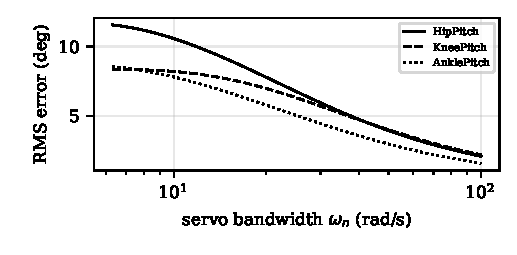
\includegraphics[width=\columnwidth]{fig/f_servo.pdf}
\caption{RMS tracking error of the left leg pitch joints against the servo bandwidth.}
\label{fig:servo}
\end{figure}

\subsection{Bandwidth budget check}
Table~\ref{tab:budget} compares \eqref{eq:budget} with the exact bandwidth that gives the target RMS error, found by root finding on \eqref{eq:erms}. The approximation is within 10 percent for tolerances up to 3 degrees, and the knee is the most demanding joint with 111 rad/s for 2 degrees and 71 rad/s for 3 degrees. These bandwidths are about 18 and 11 Hz. The two roll joints need less than half of that because their RMS velocity is 0.83 and 0.86 rad/s against 1.93 rad/s for the knee.

\begin{table}[t]
\centering
\caption{Servo bandwidth (rad/s) for a target RMS error, exact and from \eqref{eq:budget}}
\label{tab:budget}
\footnotesize
\setlength{\tabcolsep}{3pt}
\begin{tabular}{lccccc}
\toprule
 & & \multicolumn{2}{c}{$\varepsilon=2^\circ$} & \multicolumn{2}{c}{$\varepsilon=3^\circ$}\\
Joint & $\dot q_{\mathrm{rms}}$ & exact & approx. & exact & approx.\\
\midrule
Hip pitch & 1.84 & 105 & 105 & 68 & 70\\
Knee pitch & 1.93 & 111 & 111 & 71 & 74\\
Ankle pitch & 1.40 & 78 & 80 & 50 & 53\\
Hip roll & 0.83 & 45 & 48 & 29 & 32\\
Ankle roll & 0.86 & 48 & 49 & 31 & 33\\
\bottomrule
\end{tabular}
\end{table}

\subsection{Joint state view}
Figure~\ref{fig:tensor} shows the tensor $\mathbf{Q}$ of the loop as the deviation from the ready posture. Only 10 of the 22 joints move during straight walking, namely the roll and pitch joints of both legs, $n=2$ to 6 and 8 to 12. The two hip yaw pitch joints ($n=1$, 7) stay at zero, and the arms and head ($n=13$ to 22) remain at the ready posture throughout. The arm joints are therefore an unused degree of freedom of the clip. The phase portraits in Fig.~\ref{fig:phase} plot $(q_n,\dot q_n)$ for the three leg pitch joints. Each orbit is closed, as required by the closure condition, and the knee orbit touches the velocity limits at both sides, which is the graphical form of $\mathrm{VUI}\approx1$.

\begin{figure}[t]
\centering
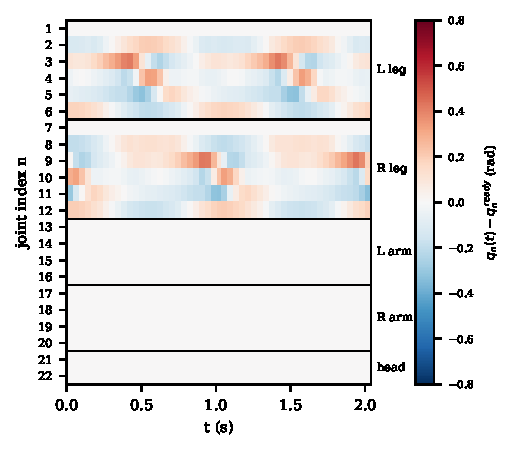
\includegraphics[width=0.9\columnwidth]{fig/f_tensor.pdf}
\caption{Joint state tensor of the walking loop, shown as the deviation $q_n(t)-q_n^{\,\mathrm{ready}}$ for all 22 joints over 2.04 s.}
\label{fig:tensor}
\end{figure}

\begin{figure}[t]
\centering
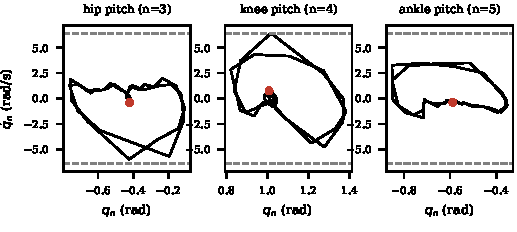
\includegraphics[width=\columnwidth]{fig/f_fase.pdf}
\caption{Phase portraits of the left leg pitch joints. The dashed lines are the velocity limits of the model and the dot marks frame 0.}
\label{fig:phase}
\end{figure}

\subsection{Kinematic stride estimate}
Equation \eqref{eq:fk} applied to the loop gives the foot position relative to the hip, shown in Fig.~\ref{fig:fk}. The sole stays flat within $0.06^\circ$ at every frame, so \eqref{eq:flat} holds along the whole clip, and the vertical foot excursion is 22 mm. During stance the foot moves backward relative to the hip by 0.0805 m on the left and 0.0807 m on the right, and this is the distance the torso advances per gait period if the foot does not slip. The measured advance is 0.18 m per 2.04 s, which is 0.09 m per period, so the planar estimate is about 10.5 percent low. The sagittal model ignores the lateral sway of the hip roll joints and the inclined hip axis, and the stance detection threshold of 2 mm is also arbitrary, so agreement within about 11 percent is a reasonable outcome for a model with no dynamics.

\begin{figure}[t]
\centering
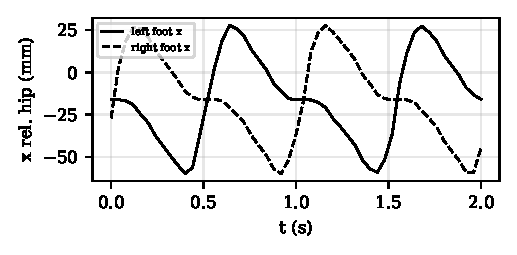
\includegraphics[width=\columnwidth]{fig/f_fk.pdf}
\caption{Foot position relative to the hip from the forward kinematics \eqref{eq:fk}, over the 2.04 s loop.}
\label{fig:fk}
\end{figure}

\section{Reconciliation with Simulation}
\label{sec:valid}
The controller was run in Webots R2025a with a 20 ms basic time step. Table~\ref{tab:meas} lists the displacement and heading change of each primitive, measured in simulation by the evaluator of the controller. The walking loop advances 0.18 m in 2.04 s, a mean speed of 0.088 m/s. The yaw pulse of \eqref{eq:pulse} commands $14.3^\circ$ of hip yaw and produces $+17^\circ$ of heading change to the left and $-13^\circ$ to the right, so the pulse gain is $G_L=1.19$ on the left and $G_R=0.91$ on the right. The asymmetry index $(G_L-G_R)/(G_L+G_R)=0.13$ indicates that the gait amplifies a left pulse and attenuates a right pulse, which a calibrated controller could correct by using the amplitudes $\psi/G_L$ and $\psi/G_R$ for a desired heading change $\psi$.

Turning in place uses the scaling $\mathcal{S}_\kappa$ applied to the 40 degree clip. The measured heading changes of $11^\circ$, $20.7^\circ$, and $39^\circ$ at $\kappa=0.25$, $0.5$, and $1$ are fitted by $\psi\approx39.7\,\kappa$ degrees through the origin, with residuals of $+1.1^\circ$, $+0.9^\circ$, and $-0.7^\circ$, so the scaling is a usable open loop heading actuator.

\begin{table}[t]
\centering
\caption{Measured motion primitives in Webots. The straight walk lasts 2.04 s and the turn around lasts 9.0 s}
\label{tab:meas}
\small
\begin{tabular}{lcc}
\toprule
Primitive & Disp. (m) & Heading (deg)\\
\midrule
Walk straight & $+0.18$ & 0\\
Walk, left pulse & $+0.16$ & $+17$\\
Walk, right pulse & $+0.17$ & $-13$\\
Turn left 40, 60 & 0 & $+39$, $+59$\\
Turn right 40, 60 & 0 & $-40$, $-59$\\
Turn, $\kappa=0.25$, $0.5$ & 0 & $\pm11$, $\pm20.7$\\
Turn around (9.0 s) & 0 & $+196$\\
Backward step & $-0.10$ & 0\\
Small forward & $+0.10$ & 0\\
\bottomrule
\end{tabular}
\end{table}

An automated stress test ran 32 sessions of 600 s each, covering 16 start positions and two exploration modes, for a total of 19 200 s (5.3 hours) of simulated time and 1384 m of travel. The test recorded 0 collisions and 0 falls. The effect of blending is visible in a controlled comparison. When the unmodified Webots clip is started from the upright posture, the robot falls forward after 1.2 s. The jump to the first pose asks for a knee displacement of 1.22 rad in one control step. The servo velocity limit of 6.40 rad/s then needs at least 0.19 s to follow, which is consistent with the lost balance. With the transitions of Section III the same start asks for at most 1.31 rad/s, which is 20 percent of the limit.

\section{Discussion and Limitations}
The analysis explains why a replay controller works. The command is $C^0$ everywhere, it is bounded in velocity below the servo limit apart from the knee, and its energy sits at a single stride frequency that a servo of moderate bandwidth can follow. The controller is nevertheless open loop at the joint level. It uses no feedback from the inertial unit, the foot force sensors, or the joint position sensors that are read at every step, so it cannot reject disturbances, and its robustness comes from the arena being flat. The Zero Moment Point and the linear inverted pendulum \cite{kajita2003,kajita2010} were not used to verify dynamic stability, since the center of mass trajectory was not recorded. The servo results are parametric, the NAO motor gains were not inspected, and all measurements come from simulation, not from a physical robot. The kinematic stride estimate is planar. The knee runs at its velocity limit, so the clip cannot be sped up.

Future work follows from these limits. A closed loop layer could add a feedback term to the hip and ankle pitch targets from the inertial unit, a stride length controller could use the kinematic model of \eqref{eq:fk}, and the quintic profile of Table~\ref{tab:profiles} could be tested as an alternative blend. Real hardware tests are needed before any claim of transfer.

\section{Conclusion}
The joint level gait engine of a NAO in Webots can be written as four operators on a joint state trajectory, and three closed form tools describe its budgets. Smoothstep blending is the minimum acceleration bridge between poses, the velocity utilization index and the time scaling bound show that the walking clip cannot be sped up because the right knee uses 102 percent of its limit, and the spectral bandwidth budget $2\dot q_{\mathrm{rms}}/\varepsilon$ gives about 70 to 110 rad/s for a knee error of 2 to 3 degrees RMS. The joint state views show that only 10 of 22 joints move during walking, and the hip yaw pulse has a measured left right asymmetry of 0.13. A planar kinematic model predicts the stride within 11 percent. The controller completed 5.3 hours of simulated walking without collisions or falls. The next steps are a closed loop layer on the inertial and foot force sensors, use of the idle arm joints, and tests on a physical robot.

\begin{thebibliography}{99}
\bibitem{gouaillier2009} D. Gouaillier \textit{et al.}, ``Mechatronic design of NAO humanoid,'' in \textit{Proc. IEEE Int. Conf. Robotics and Automation (ICRA)}, 2009, pp. 769 to 774.
\bibitem{vukobratovic2004} M. Vukobratovi\'c and B. Borovac, ``Zero moment point, thirty five years of its life,'' \textit{Int. J. Humanoid Robotics}, vol. 1, no. 1, pp. 157 to 173, 2004.
\bibitem{kajita2003} S. Kajita \textit{et al.}, ``Biped walking pattern generation by using preview control of zero moment point,'' in \textit{Proc. IEEE Int. Conf. Robotics and Automation (ICRA)}, 2003, pp. 1620 to 1626.
\bibitem{kajita2010} S. Kajita \textit{et al.}, ``Biped walking stabilization based on linear inverted pendulum tracking,'' in \textit{Proc. IEEE/RSJ Int. Conf. Intelligent Robots and Systems (IROS)}, 2010, pp. 4489 to 4496.
\bibitem{westervelt2003} E. R. Westervelt, J. W. Grizzle, and D. E. Koditschek, ``Hybrid zero dynamics of planar biped walkers,'' \textit{IEEE Trans. Automatic Control}, vol. 48, no. 1, pp. 42 to 56, 2003.
\bibitem{englsberger2015} J. Englsberger, C. Ott, and A. Albu-Sch\"affer, ``Three dimensional bipedal walking control based on divergent component of motion,'' \textit{IEEE Trans. Robotics}, vol. 31, no. 2, pp. 355 to 368, 2015.
\bibitem{erbatur2009} K. Erbatur and O. Kurt, ``Natural ZMP trajectories for biped robot reference generation,'' \textit{IEEE Trans. Industrial Electronics}, vol. 56, no. 3, pp. 835 to 845, 2009.
\bibitem{kofinas2015} N. Kofinas, E. Orfanoudakis, and M. G. Lagoudakis, ``Complete analytical forward and inverse kinematics for the NAO humanoid robot,'' \textit{J. Intelligent and Robotic Systems}, vol. 77, pp. 251 to 264, 2015.
\bibitem{michel2004} O. Michel, ``Webots professional mobile robot simulation,'' \textit{Int. J. Advanced Robotic Systems}, vol. 1, no. 1, pp. 39 to 42, 2004.
\bibitem{flash1985} T. Flash and N. Hogan, ``The coordination of arm movements, an experimentally confirmed mathematical model,'' \textit{J. Neuroscience}, vol. 5, no. 7, pp. 1688 to 1703, 1985.
\bibitem{astrom2001} K. J. {\AA}str\"om and T. H{\"a}gglund, ``The future of PID control,'' \textit{Control Engineering Practice}, vol. 9, no. 11, pp. 1163 to 1175, 2001.
\bibitem{denavit1955} J. Denavit and R. S. Hartenberg, ``A kinematic notation for lower pair mechanisms based on matrices,'' \textit{J. Applied Mechanics}, vol. 22, no. 2, pp. 215 to 221, 1955.
\bibitem{bobrow1985} J. E. Bobrow, S. Dubowsky, and J. S. Gibson, ``Time optimal control of robotic manipulators along specified paths,'' \textit{Int. J. Robotics Research}, vol. 4, no. 3, pp. 3 to 17, 1985.
\bibitem{pham2018} H. Pham and Q.-C. Pham, ``A new approach to time optimal path parameterization based on reachability analysis,'' \textit{IEEE Trans. Robotics}, vol. 34, no. 3, pp. 645 to 659, 2018.
\bibitem{webotsmanual} Cyberbotics Ltd., \textit{Webots Reference Manual}, Motor node, 2025.
\end{thebibliography}

\end{document}
